%----------------------------------------------------------------------------
\chapter{Megvalósítás}
%----------------------------------------------------------------------------

{\color{red} Először valami bla-bla}



%----------------------------------------------------------------------------
\section{Alapok}
%----------------------------------------------------------------------------



Az OpenCV remek keretrendszer, rengeteg gyakran használt algoritmust implementáltak benne, viszont felépítését tekintve procedurális. Jelen feladatom megoldása során törekedtem az átlátható és jól struktúrált kód kialakítására, így ahol szükségesnek éreztem osztályokba szerveztem a logikát.

OpenCV-ben a legtöbb adatot egy mátrix (\texttt{cv::Mat}) adattípus reprezentál, ide értve a matematikai értelemben vett mátrixokat és a képeket is. Egy ilyen mátrix lényegében egy kétdimenziós tömb, melynek elemei lehetnek skalárok, de több-dimenziós vektorok is (több csatornás).

Elsőnek a \texttt{Camera} osztály, és annak konkrét implementáció készültek el, elfedve azt, hogy éppen a valódi kamerából kérünk le képkockákat, vagy fájlból olvassuk ki azokat. Ebből adódóan a \texttt{RealCamera} lényegében becsomagolja az OpenCV-s \texttt{VideoCapture} osztályt, és a \texttt{Camera} absztakt osztály közös interfészt nyújt a fájlból történő olvasáshoz is a \texttt{FakeCamera} számára. Ez főleg a tesztelés során volt hasznos, hogy egy adott jelenetet elég volt egyszer felvenni, és utána azt tudtam bemenetként használni. Az osztálydiagram \aref{fig:cd:camera}. ábrán látható.

A \texttt{cameraMatrix} attribútum jelöli a \textit{kamera-mátrix}ot és a \texttt{distCoeffs} attribútum a torzítási együtthatókat (lásd \aref{sec:pinhole}. szekció). Mivel ezek egy kamerára nézve időben állandóak, ezért csak egyszer kell őket meghatározni. A \texttt{readCalibration()} metódus szolgál ezek külső fájlból történő beolvasásukra. Miután rendelkezésre állnak ezek a paraméterek, akkor a \texttt{readUndistorted()} metódus segítségével olvashatok be rektifikált képet. A másik 3 metódus megfelel az azonos nevű metódusoknak a \texttt{cv::VideoCapture} osztályban \cite{cv_video}, ahol a \texttt{grab()} egy képkockát szerez az eszköztől, de nem olvassa (dekódolja) ki, míg a \texttt{retrieve()} ezt teszi. Ezt a kombinációt több kamerás rendszernél célszerű használni, úgy, hogy először mindegyik kamerán meghívjuk a \texttt{grab()}-et, majd utána lekérjük a képeket (amely művelet időigényes). Ezzel a módszerrel érhető el, hogy időben a lehető legközelebb legyenek a különböző kamerákból lekért képkockák egymáshoz. A \texttt{read()} a kettőt kombinálja kényelmi szempontból.

\begin{figure}[tbh]
\centering

\begin{tikzpicture} 

\begin{abstractclass}[text width=7 cm]{Camera}{0, 0}
\attribute   {+ cameraMatrix : Mat}
\attribute   {+ distCoeffs : Mat}

\operation   {+ readCalibration(fileName) : void}
\operation   {+ readUndistorted(outputImg) : void}
\operation[0]{+ grab() : void}
\operation[0]{+ retrieve(outputImg) : void}
\operation[0]{+ read(outputImg) : void}
\end{abstractclass}

\begin{class}[text width=5 cm]{RealCamera}{-4, -5.5}
\inherit{Camera}
\operation{+ grab() : void}
\operation{+ retrieve(outputImg) : void}
\operation{+ read(outputImg) : void}
\end{class}

\begin{class}[text width=5 cm]{DummyCamera}{4, -5.5}
\inherit{Camera}
\operation{+ grab() : void}
\operation{+ retrieve(outputImg) : void}
\operation{+ read(outputImg) : void}
\end{class}

\end{tikzpicture}

\caption{Osztályok a kamerához kezeléséhez \label{fig:cd:camera}}
\end{figure}


\section{Kalibráció}

Elsőként meg kell határoznom a kamerák már előbb is említett belső paramétereit. A módszert \aref{sec:pinhole}. szekcióban mutattam be, a következőkben ennek megvalósítását tárgyalom. Ehhez készült egy segédosztály \texttt{Calibration} néven, melynek feladata, hogy kellő információ után meghatározza a kamera-mátrixot és a torzítási együtthatókat és kiírja ezeket egy fájlba, hogy azt vissza tudjuk olvasni.

\begin{figure}[tbh]
\centering

\begin{tikzpicture} 

\begin{class}[text width=7 cm]{Calibration}{0, 0}
\attribute{- camera : Ptr<Camera>}
\attribute{- corners : vector<vector<Point2f>{}>}
\attribute{- cameraMatrix : Mat}
\attribute{- distCoeffs : Mat}

\operation{+ Calibration(camera)}
\operation{+ acquireFrame() : bool}
\operation{+ calibrate() : void}
\operation{+ save(fileName) : void}
\end{class}

\end{tikzpicture}

\caption{\texttt{Calibration} osztály \label{fig:cd:calibration}}
\end{figure}

Konstruktorban át kell neki adni a kamerára vonatkozó pointert, amitől a képeket kell majd lekérnie. Az \texttt{acquireFrame()} metódus szerepe, hogy a kamera aktuális képkockáját megszerezze, megkeresse a képen a sakktáblát, és a sakktábla sarokponjaihoz tartozó koordinátákat a \texttt{corners} listához fűzze. Visszatérési értékben jelzi, hogy az adott képen sikeres volt-e a detekció. Belsőleg a \texttt{cv::findChessboardCorners()} OpenCV-s függvényt hívja, amelynek átadva egy fekete-fehér képet, megkapható a képen látható sakktábla sarokpontjainak képpontjai. Kellő képkocka után a \texttt{calibrate()} metódus segítségével a kérdéses két mátrix (\texttt{cameraMatrix}, \texttt{distCoeffs}) kiszámolható. Itt a \texttt{cv::calibrateCamera()} függvényt hívom segítségül, melynek két fontos bemeneti paraméterét emelem ki: az sarokpontok valóvilágbeli koordinátái, és a képeken detektált képpontjai sorfolytonosan (\texttt{corners}). A valóvilágbeli $(x, y, z)$ koordinátákat az egyszerűség kedvéért úgy választottam, hogy $z \equiv 0$, és $x$ valamint $y$ egész számok úgy, hogy a sakktábla bal felső sarka $(0, 0, 0)$, jobb alsó sarka pedig -- $9\times 6$-os sakktáblát használva -- $(9, 6, 0)$. A \texttt{save()} pedig kimenti a paramétereket olyan formátumban, amiből a \texttt{Camera::readCalibration()} vissza tudja olvasni.


\subsection{Kamerák pozíciójának meghatározása világkoordinátákban}


Rögzített kamerák révén lehetőségem adódik, hogy előre meghatározzam a kamerák pozícióját és nézőpontjuk irányát. Erre egy kalibrációs objektumot használok, szintén egy sakktáblát. Amennyiben megadom a sakktábla sarokpontjainak koordinátáit az előbbiekkel egyező módon, akkor a sakktábla rögzítésével a térben, a koordinátarendszert is rögzítem. 

Az OpenCV-ben erre a célra van a \texttt{solvePnP} függvény, mely 3D-2D pont-összerendelésekből, kiszámolja a forgatási és eltolási vektort, amik együttesen megadják a transzformációt a model-koordinátarendszerből a kamera koordinátarendszerébe. Ezen funkciót a \texttt{CameraPoseCalculator} osztály ágyazza be, és a két vektort pedig a \texttt{CameraPose} csomagolja össze egy perzisztálható osztályba, lásd \aref{fig:cd:pose}. ábra.

\begin{figure}[tbh]
\centering

\begin{tikzpicture} 

\begin{class}[text width=5.3 cm]{CameraPoseCalculator}{-8.5, -0.50}
\attribute{- cam : Ptr<Camera>}

\operation{+ CameraPoseCalculator(cam)}
\operation{+ calculator() : bool}
\end{class}

\begin{class}[text width=5 cm]{CameraPose}{0, 0}
\attribute{+ rvec : Mat}
\attribute{+ tvec : Mat}

\operation{+ save(fileName) : void}
\operation{+ load(fileName) : void}
\operation{+ getRT() : Matx34d}
\end{class}

\aggregation{CameraPoseCalculator}{cameraPose~~~~~~~~~~}{1}{CameraPose}

\end{tikzpicture}

\caption{\texttt{CameraPoseCalculator} és \texttt{CameraPose} osztály \label{fig:cd:pose}}
\end{figure}

A \texttt{CameraPoseCalculator} osztály megkapja konstruktor argumentumaként annak a kamerára mutató pointerét, amelynek a külső paramétereit (forgatási és eltolási vektor, lásd \ref{sec:pinhole}. szekció vége) ki kell számolnia. A konkrét művelet végrehajtásáért a \texttt{calculator()} metódus felelős, amely a kamerától lekér egy képkockát, megkeresi rajta a sakktáblát, majd meghívja a \texttt{cv::solvePnP()} függvényt. Visszatérési értékben jelzi, hogy sikeres volt-e a detekció, ha igen, akkor lekérhető tőle a \texttt{CameraPose} példány. Ez utóbbi a \texttt{save()} és \texttt{load()} metódusokkal elmenthető és visszatölthető, így ameddig a kamerát nem mozgatjuk el, ez újra felhasználható. A \texttt{getRT()} metódus a forgatási vektorból forgatási mátrixot csinál (Rodrigues-féle forgatási formula \cite{camera-calib-3d}) és összefűzi azt az eltolási vektorral egy $3\times 4$-es $\Big(\,\mathbf{R}\,|\,\mathbf{t}\,\Big)$ forgatás-eltolás mátrixba.

A kamera külső paramétereinek meghatározása után már minden információ adott, hogy 3D-s pontok 2D-s vetületeit meg tudjam határozni a \texttt{cv::projectPoints()} függvény felhasználásával. \Aref{fig:pose}. ábrán látható, hogy egy a sakktábla síkjába rajzolt négyzetrács, melynek egyik jelölt pontja a világ-koordinátarendszer origója.

\begin{figure}[tbh]
\centering
\begin{subfigure}[b]{.49\linewidth}
	\centering
	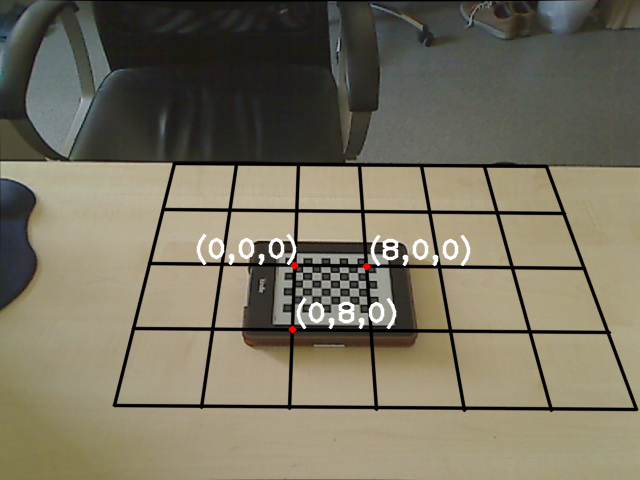
\includegraphics[width=205pt]{figures/pose0_180.png}
	\caption{Bal oldali kamera}
  \end{subfigure}
\begin{subfigure}[b]{.49\linewidth}
	\centering
	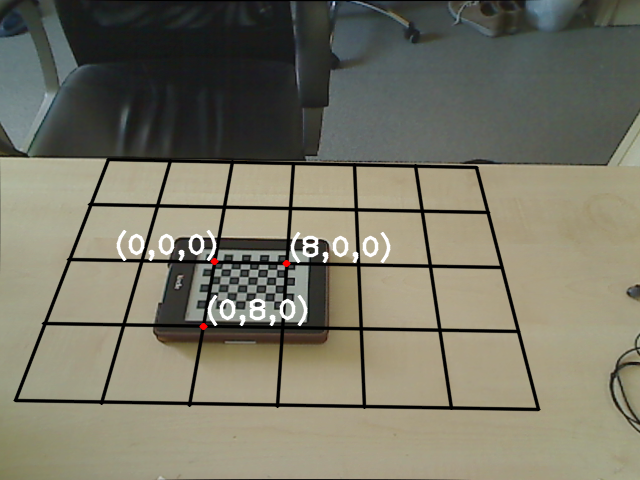
\includegraphics[width=205pt]{figures/pose1_180.png}
	\caption{Jobb oldali kamera}
  \end{subfigure}
\caption{Világ-koordinátarendszer jelölése a képeken \label{fig:pose}}
\end{figure}

%----------------------------------------------------------------------------
\section{Objektum detekció}
%----------------------------------------------------------------------------



\Aref{sec:obj_detection}. szekcióban leírtam a mozgó objektumok detekciójának egy lehetséges megközelítését. A lényege, hogy egy háttér modellt építünk, és így mindig aktuálisan lekérhető az előtérhez tartozó maszk, ami kijelöli a mozgó objektumokat. A probléma megoldása két fázisra bontható: először egyetlen objektumot keresek és detektálok, majd később több mozgó objektumot is.

Mindkét fázisnak közös része a már említett modellépítés, melyhez az OpenCV-ben megtalálható \texttt{BackgroundSubtractorMOG2} osztályt \cite{opencv-mog} hívom segítségül. Példányosítás után a modell építése, és az aktuális maszk kinyerése az \texttt{apply} metódussal történik. \Aref{fig:my_mog2}. ábrán látható a kinyerhető maszkra egy példa.

\begin{figure}[tbh]
\centering
\begin{subfigure}[b]{.32\linewidth}
	\centering
	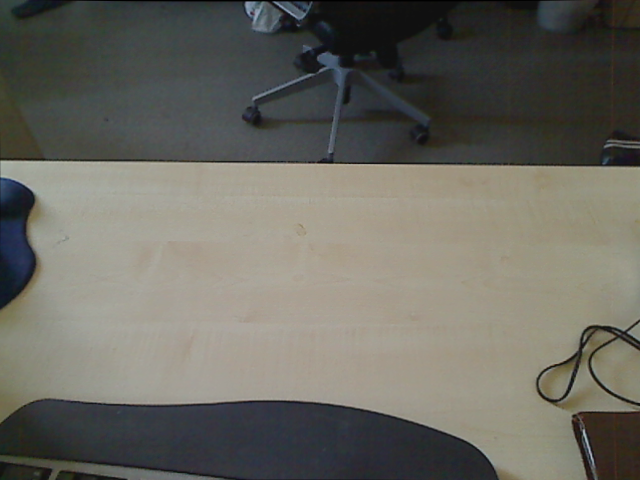
\includegraphics[width=137pt]{figures/image230.png}
	\caption{Statikus kép -- ,,háttér''}
  \end{subfigure}
\begin{subfigure}[b]{.32\linewidth}
	\centering
	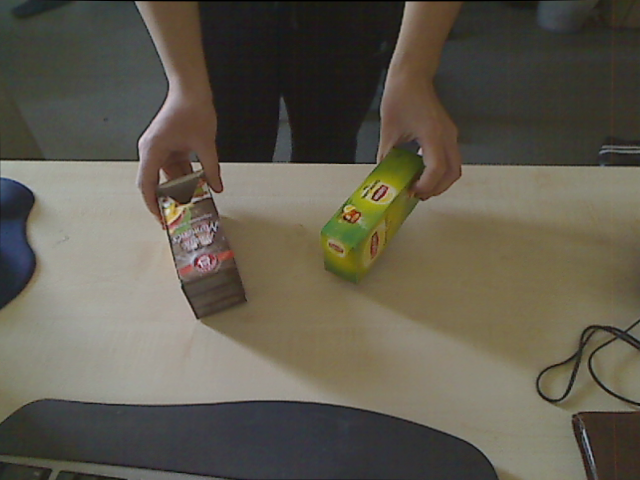
\includegraphics[width=137pt]{figures/image343.png}
	\caption{Mozgó képsor egy képe}
  \end{subfigure}
\begin{subfigure}[b]{.32\linewidth}
	\centering
	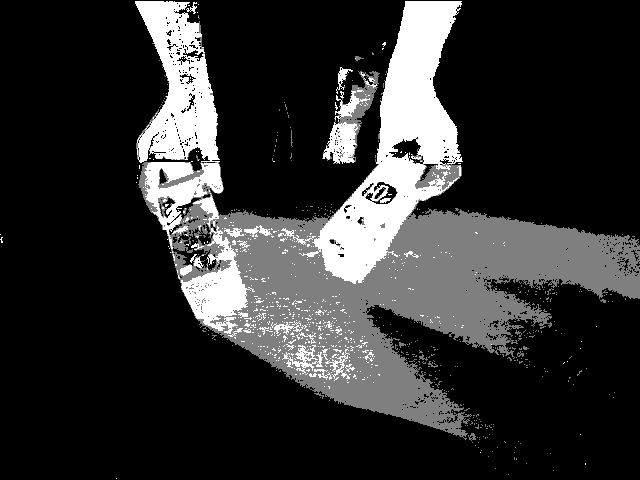
\includegraphics[width=137pt]{figures/mask343.png}
	\caption{Kapott előtér maszk}
  \end{subfigure}
\caption{Példa az előtér maszkra \label{fig:my_mog2}}
\end{figure}

Megfigyelhető, hogy a maszk nem pusztán bináris, hanem azt is jelzi, amit az algoritmus árnyéknak gondol. A zajt a maszkon az erózió-dilatáció morfológiai módszerek segítségével tudjuk csökkenteni. Előbbi a kisméretű zajokat tünteti el, utóbbi pedig a lyukakat szünteti meg. OpenCV-ben ezek implementációi a \texttt{dilate} és \texttt{erode} függvények. Előbbi az adott pixelt a környezetében (amit egy kernel ír le) lévő maximális, míg utóbbi a minimális értékkel helyettesít. Én egy erózió-dilatáció-erózió lépéssorozatot használok: először az apróbb szemcsék szűnnek meg, utána a lyukak. Az utolsó erózió szerepe, hogy az objektumok szélén a dilatáció miatt jelentkező növekedést megszűntesse. Ennek eredménye látható \aref{fig:erosion_dilation}. ábrán.

\begin{figure}[tbh]
\centering
\begin{subfigure}[b]{.49\linewidth}
	\centering
	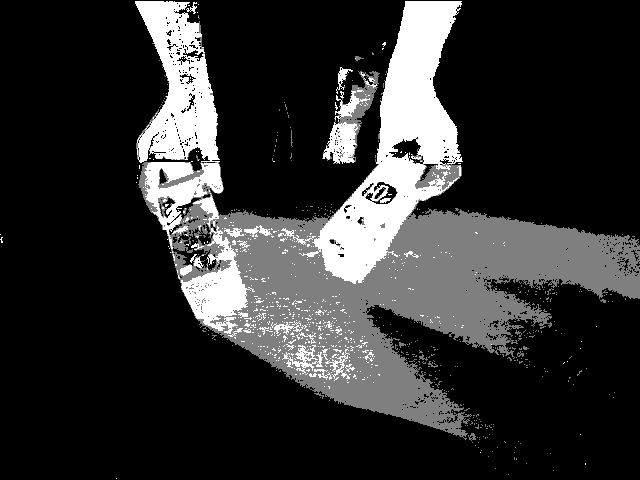
\includegraphics[width=205pt]{figures/mask343.png}
	\caption{Eredeti}
  \end{subfigure}
\begin{subfigure}[b]{.49\linewidth}
	\centering
	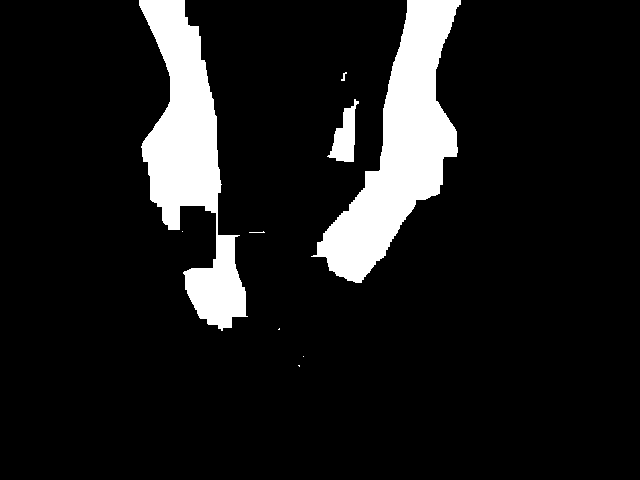
\includegraphics[width=205pt]{figures/mask343_fixed.png}
	\caption{Árnyékok kivétele és zajcsökkentés után}
  \end{subfigure}
\caption{Előtér maszk zajmentesítése \label{fig:erosion_dilation}}
\end{figure}

Megfigyelhető, hogy a bal oldali dobozhoz tartozó maszk része annyira zajos volt, hogy a nagy lyuk nem szűnt meg, míg a kevésbé zajos jobb oldali doboz rendben megmaradt. A maszkot alkalmazva az eredeti képre \aref{fig:mask_applied}. ábrán látható, hogy egy bizonyos hibahatáron belül sikeresnek tekinthető a mozgó részlet kijelölése.

\begin{figure}[tbh]
\centering
\begin{subfigure}[b]{.49\linewidth}
	\centering
	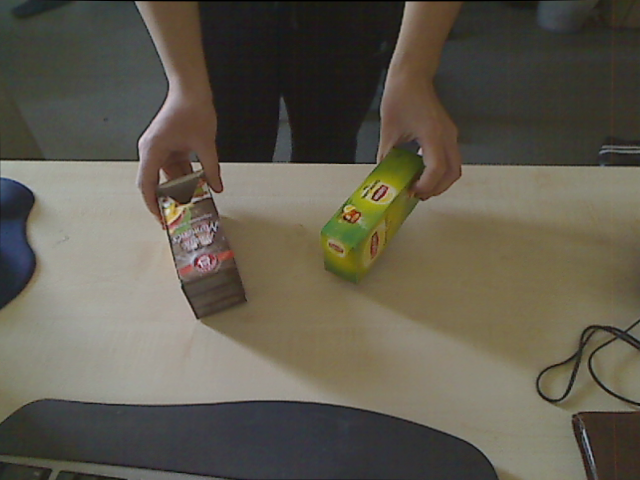
\includegraphics[width=205pt]{figures/image343.png}
	\caption{Eredeti kép}
  \end{subfigure}
\begin{subfigure}[b]{.49\linewidth}
	\centering
	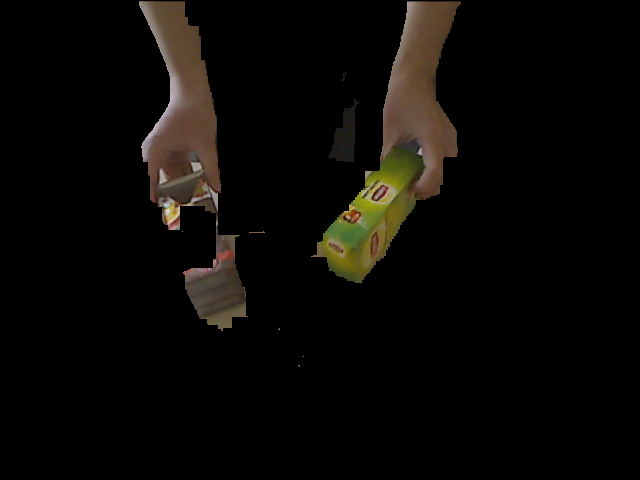
\includegraphics[width=205pt]{figures/mask343_applied.png}
	\caption{A detektált előtér}
  \end{subfigure}
\caption{Előtér maszk alkalmazás az eredeti képre \label{fig:mask_applied}}
\end{figure}

\subsection{Egyetlen objektum detekciója}

Kezdetben azzal az egyszerűsítéssel élek, hogy a képen csak egyetlen mozgó objektumot detektálok, mégpedig azt, amelyik a legnagyobb részt foglalja el a képen. Ez nagyban egyszerűsíti a dolgokat, mert ahogy majd látni fogjuk a következő szekcióban, az optikai folyam meghatározására szükség lesz a képeken látható \textit{blob}ok (egy objektumhoz tartozó egybefüggő rész a képen) párosításra a kamerák képein. Mivel összesen egy blobot jelölök ki a képeken, ezek párosítása triviális, és nagy valószínűséggel ugyanazon objektumhoz tartoznak majd.

Ezen logikát egy \texttt{SingleObjectSelector} osztályban implementáltam. Egyetlen metódusa van, amely paraméterül a képet és a (zajcsökkentett) előtér maszkot várja, visszatérési értéke pedig a kép azon része, melyet a maszk legnagyobb területű blobja jelöl ki. Ez utóbbit a \texttt{lastMask}-ban le is lehet kérdezni, és a későbbi könnyebb feldolgozás érdekében az ehhez tartozó befoglaló téglalapot is (\texttt{lastBoundingRect}). A megoldásom az OpenCV \texttt{findContours()} függvényére épít. Segítségével lekérem a maszkon található legkülső kontúrokat (a belső lyukakat is az objektum részének tekintem), és ezek közül azt választom, amelyiknek a legnagyobb a területe (ehhez a \texttt{cv::contourArea()}-t hívom segítségül).

\begin{figure}[tbh]
\centering

\begin{tikzpicture} 

\begin{class}[text width=10 cm]{SingleObjectSelector}{0, 0}
\attribute{+ lastMask : Mat}
\attribute{+ lastBoundingRect : Rect}

\operation{+ selectUsingContourWithMaxArea(img, mask) : Mat}
\end{class}

\end{tikzpicture}

\caption{\texttt{SingleObjectSelector} osztály \label{fig:cd:singleobjectselector}}
\end{figure}

\Aref{fig:maxArea}. ábrán látható az előbbiekben bemutatott maszkhoz meghatározott kontúrok és teli fehérrel a kiválasztott legnagyobb blob.

\begin{figure}[tbh]
    \centering
    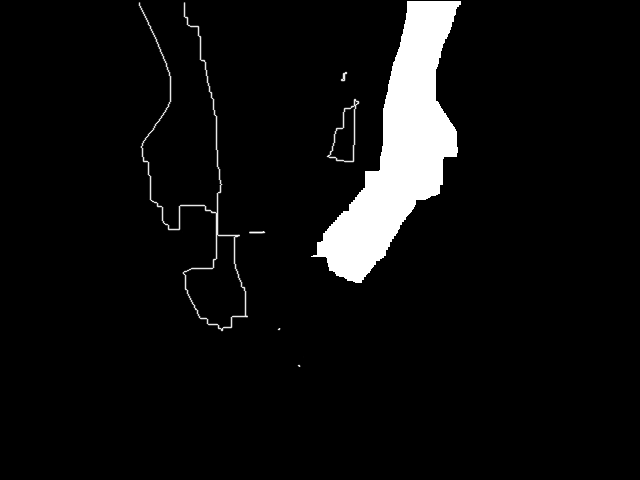
\includegraphics[width=250pt]{figures/mask343_contours.png}
    \caption{Legnagyobb blob kijelölése \label{fig:maxArea}}
\end{figure}

\subsection{Több objektum detekciója, párosítás a kamerák képein}

{\color{red} TODO: SURF + FLANN, fullos osztályok a matchingekhez}



%----------------------------------------------------------------------------
\section{Optikai folyam meghatározása}
%----------------------------------------------------------------------------


\Aref{chapter2}. fejezetben bemutattam a sűrű optikai folyamok meghatározására Gunner Farnebäck módszerét. Ennek alkalmazását, valamint OpenCV-ben történő implementációjáról lesz szó ebben a részben.

A \texttt{cv::calcOpticalFlowFarneback()} függvény segítségével két képkockán meghatározhatom az optikai folyamot. Az algoritmus jellegéből adódóan nagy mozgásokat nem tud követni, de az implementáció támogatja a piramis-módszert, azaz nagy mozgások esetén a képeket több lépcsőben kicsinyíti, így az eredeti képen lévő nagy mozgások kisebbek lesznek, a kicsik pedig eltűnnek. A futási idő természetesen függ a kép méretétől, így fontos, hogy kihasználjuk az objektum maszkjából nyerhető információt.

A következőkben \aref{fig:of_original}. ábrán látható két képkocka lesz a kiinduló állapot, már az előbbiekben bemutatott előtér maszk által kijelölve. A képkockák két olyan kamera beállításal készültek, ahol a két kamera képsíkja nagyjából egybe esik (egy irányba néznek), és csak víszintes irányban vannak egymáshoz képest eltolva.

\begin{figure}[tbh]
\centering
\begin{subfigure}[b]{.49\linewidth}
	\centering
	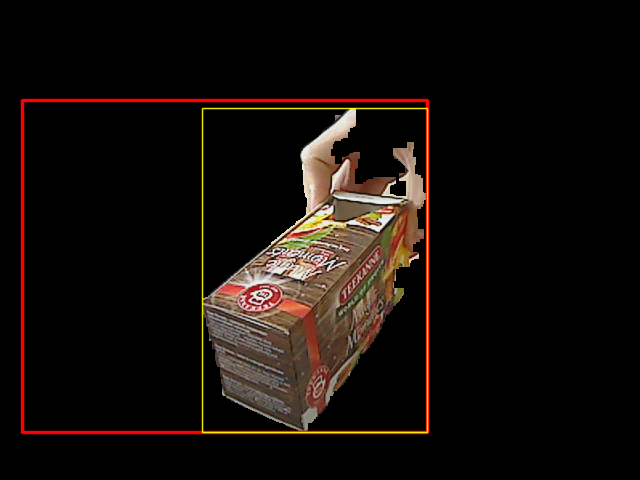
\includegraphics[width=205pt]{figures/of_img_left_framed.png}
  \end{subfigure}
\begin{subfigure}[b]{.49\linewidth}
	\centering
	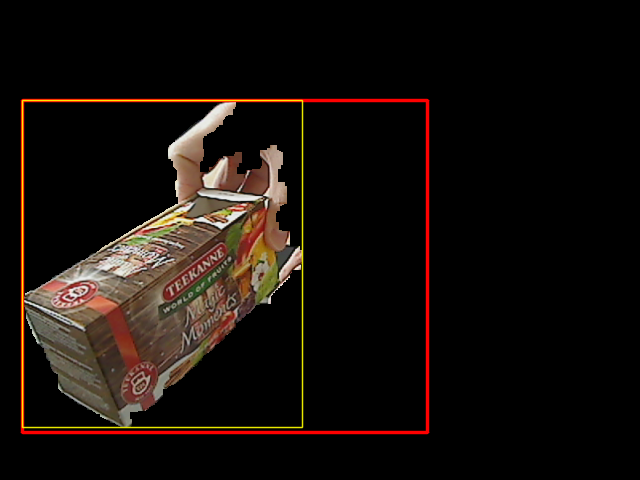
\includegraphics[width=205pt]{figures/of_img_right_framed.png}
  \end{subfigure}
\caption{Bal és jobb kamera által látott objektum kijelölve; a sárga keretek jelölik az objektumok befoglaló téglalapjait, a piros pedig ezen téglalapokat tartalmazó legkisebb területű téglalapot \label{fig:of_original}}
\end{figure}

Első megközelítésem, hogy a két objektum befoglaló téglalapját tekintem, és veszem azt a téglalapot, mely a legkisebb területű azok közül, amely mindkettőt tartalmazza. Kivágva ezt a téglalapot a két képből, két egyforma méretű képrészletet kapok, melyek külön-külön tartalmazzák a teljes objektumot. Ez látható \aref{fig:of_original}. ábrán pirossal jelölve. Erre a két részletre számolva optikai folyamot, 7 646 darab vektort kaptam, melyek közül néhányat vizualizáltam \aref{fig:bad0}. ábrán. A vektorok kezdő és végpontjaiból alkotok pontpárokat, ezeket tekintem egymásnak megfelelő pontoknak a két képen. Jól látható, hogy a kevés kirajzolt pontpárból egyik sem tekinthető jónak, mert a doboz különböző lapjaihoz tartozó pontok. Ez a nagy elmozdulás miatt van, hiába a piramis módszer, nem használható a végeredmény.

\begin{figure}[tbh]
\centering
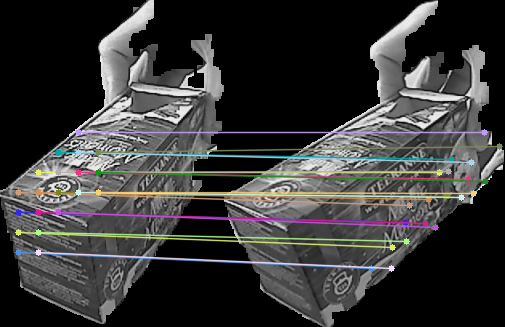
\includegraphics[width=300pt]{figures/vis_bad_0.png}
\caption{Első megközelítés (36 958 vektor) \label{fig:bad0}}
\end{figure}

A következő lépésem, hogy meghatározom azt a vektort, amivel eltolva az egyik képet, az egymásnak megfelelő képpontok elmozdulásai a lehető legkisebbek lesznek. Ehhez először szükségem van néhány egymásnak megfelelő pontpárra.

A SURF (Speeded Up Robust Features \cite{surf}) segítségével a képeken jellegzetes pontokat detektálhatunk és kiszámolhatunk ezek leíró vektorait, mely a pontokat és azok környezetét skála- és forgatás-invariáns módon azonosítja. Utóbbi tulajdonságra szükségünk is van, hiszen az objektumokról a képek más szögben és irányban készülnek. Ennek az implementációját OpenCV-ben a \texttt{cv::SURF} \cite{opencv-surf} osztályban találhatjuk, amely mind a pontok detekcióját, mind azok leírásának módját tartalmazza és megvalósítja.

Miután mindkét képen kinyertem a leíró vektorokat ezeket párosítanom kell. Ehhez a FLANN (Fast Approximate Nearest Neighbor Search Library \cite{flann_pami_2014}) könyvtárat használom, melyhez OpenCV-ben is elkészült az interfész \cite{opencv-flann}. Ennek segítségével gyorsan tudunk több dimenziós vektortérben egy vektorhoz (előzőkben kiszámolt leírók) megkeresni a hozzá legközelebbi vektort.

{\color{red} Valami kis implementációs dolog az osztályokról}

Annak ellenére, hogy a leírók nagyon hasonlóak, a párosításban szerepelhetnek rossz párok. Ismétlődő mintáknál előfordul, hogy két különböző pont képe nagyon közeli leíróvektort kap. Ezen a már használt epipoláris ($\mathbf{u}'^T \mathbf{F} \mathbf{u} = 0$) kényszert érvényesítve segítettem, azaz azokat a párokat kiszűrtem ahol az előző érték egy küszöbértéknél nagyobb. \Aref{fig:flann-matched}. ábrán látható a szűrés előtti és utáni párosítások.

\begin{figure}[tbh]
\centering
\begin{subfigure}[b]{.49\linewidth}
	\centering
	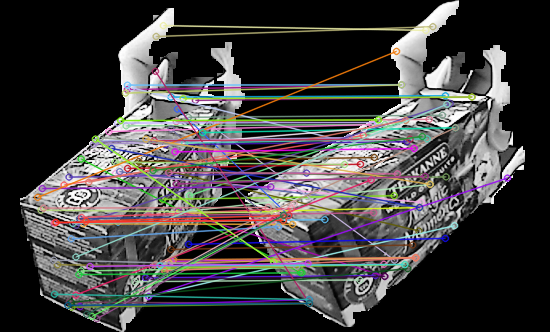
\includegraphics[width=205pt]{figures/matches_flann.png}
  \end{subfigure}
\begin{subfigure}[b]{.49\linewidth}
	\centering
	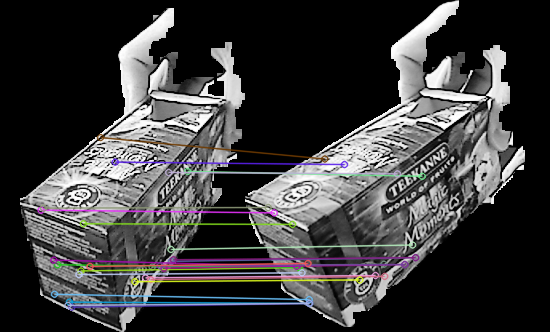
\includegraphics[width=205pt]{figures/matches_f.png}
  \end{subfigure}
\caption{Szűrés előtti (100 db) és utáni (25 db) párosítások a SURF és FLANN együttes használatával \label{fig:flann-matched}}
\end{figure}

Ezek után a párosítások jelentette vektorokból kell meghatároznom azt a vektort, amellyel az egyik képet eltolva az összetartozó pontok közötti távolság minimális. Azaz

\[\min_{\mathbf{v}(x, y)} \sum_{i=1}^{n} |\mathbf{v} - \mathbf{d_i}|\]

ahol $\mathbf{d_1}(x_1, y_1), \mathbf{d_2}(x_2, y_2), \ldots \mathbf{d_n}(x_n, y_n)$ a párosításban szereplő pontok közti távolságvektorok. Vagyis:

\[\min_{x, y} \sum_{i=1}^{n} \sqrt{(x-x_i)^2 + (y-y_i)^2}\]

{\color{red}Mivel a gyökvonás monoton, és a gyökvonás ezért a minimalizálásnál elhagyhatjuk. Így viszont ez megfogalmazható legkisebb négyzetek problémának, ami megoldható szinguláris érték szerinti felbontással.} \Aref{fig:shifted}. ábrán látható az eltolás előtt és után az objektum helyzete a két képen.

\begin{figure}[tbh]
\centering
\begin{subfigure}[b]{.49\linewidth}
	\centering
	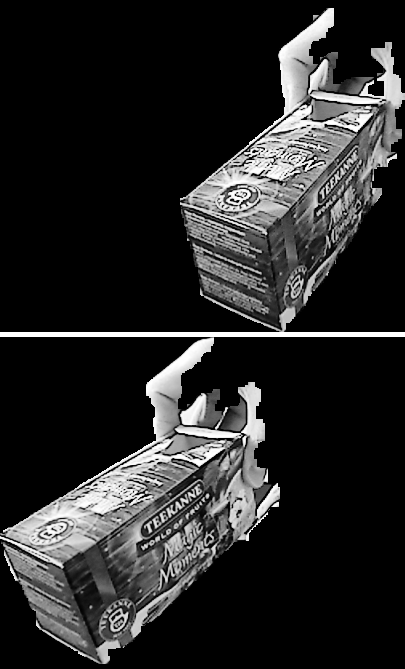
\includegraphics[height=205pt]{figures/before_shift.png}
  \end{subfigure}
\begin{subfigure}[b]{.49\linewidth}
	\centering
	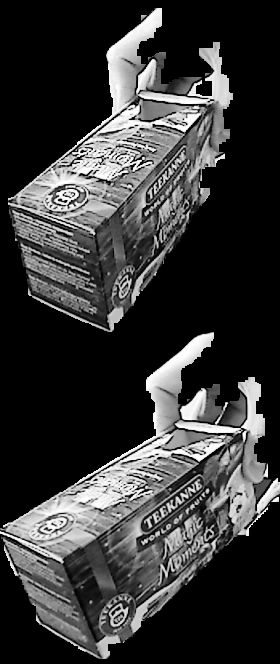
\includegraphics[height=205pt]{figures/after_shift.png}
  \end{subfigure}
\caption{Az objektum elhelyezkedése a kamerák képein (egymás alatt a két kamera képe) eredetileg és a kiszámolt vektorral való eltolás után. \label{fig:shifted}}
\end{figure}

Optikai folyamok számítása esetén két jelenséget nem szabad figyelmen kívül hagynunk: egyik a textúrázatlanság, a másik pedig a kitakart pontok problémája. Ezeken az optikai folyam rektifikációja segíthet. \cite{optical-flow-rectification}-ban You Yang és társai egy bináris függvényt javasolnak a textúrázatlanság eldöntésére:

\[
    \zeta(\Omega_\mathbf{X})= 
\begin{cases}
    0,              & \text{ha } \sigma(I_{\forall \mathbf{Y}\in\Omega_\mathbf{X}} - I_\mathbf{X}) < \varepsilon_\Omega\\
    1,              & \text{különben}
\end{cases}
\]

ahol $\Omega_\mathbf{X}$ jelöli $\mathbf{X}$ képpont egy környezetét, $I_\mathbf{X}$ az $\mathbf{X}$ pont intenzitását, $\sigma(.)$ a szórás-operátort egy halmazra nézve, valamint $\varepsilon_\Omega$ egy küszöbértéket, ami konstans. Úgy találták, hogy $\varepsilon_\Omega = 6$ választással jó eredményeket értek el, így én is ezt használtam. A mintaképek pontjaira kiszámolve ezt a függvényt, \aref{fig:textures}. ábrán látható maszkokat kaptam.

\begin{figure}[tbh]
\centering
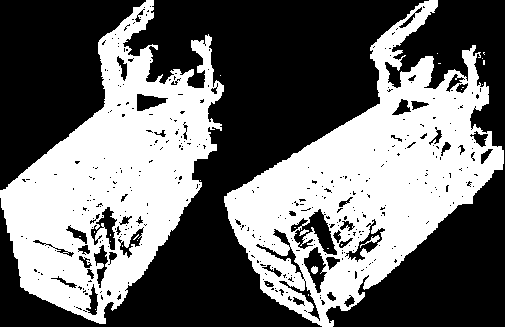
\includegraphics[width=300pt]{figures/textures.png}
\caption{$\zeta$ függvény alkalmazva az objektum összes pontjára \label{fig:textures}}
\end{figure}

{\color{red}A kitakart pontok kiszűrésére én \cite{optical-flow-rectification}-től eltérő megközelítést alkalmaztam.} Legyen két képkocka $K_1$ és $K_2$, valamint $F_{1, 2} = \mathcal{F}(K_1, K_2)$ és $F_{2, 1} = \mathcal{F}(K_2, K_1)$, ahol $\mathcal{F}$ jelöli két képkocka közti optikai-folyam operátort, melynek eredménye egy vektormező ($F_{1, 2}, F_{2, 1} : \mathbb{R}^2 \rightarrow \mathbb{R}^2$). Gondoljuk meg, hogy ha $x\in K_1$ és $x + F_{1,2}(x) = x' \in K_2$, akkor $x' + F_{1,2}(x') \approx x \in K_1$, vagyis ha egy $x$ pont $K_1$-ről $K_2$-re az $x'$ pontba mozog, akkor visszafelé nézve $x'$ pontnak ideális esetben $x$ pontba kell, hogy mozogjon. Tehát oda-vissza számolva 1-1 optikai folyamot a kitakart pontokat kiszűrhetjük, hiszen a másik irányban nem fogjuk megtalálni a párosítást.

{\color{red} Valami implementációs dolog az egészről?}

Miután az előzőekben leírtakat felhasználtam és implementáltam, \aref{fig:vis_full}. ábrán kiemeltem néhány párosítást. Szabad szemmel is jól látható, hogy egész pontos párosításokat kaptam, összesen 16 841-et, tehát ennyi pontpárt tudunk majd a háromszögeléshez felhasználni. Vessük össze ezt a SURF leírókka történő párosításnál nyert 100, majd abból meghagyott 25 párral, számottevő a különbség.

\begin{figure}[tbh]
\centering
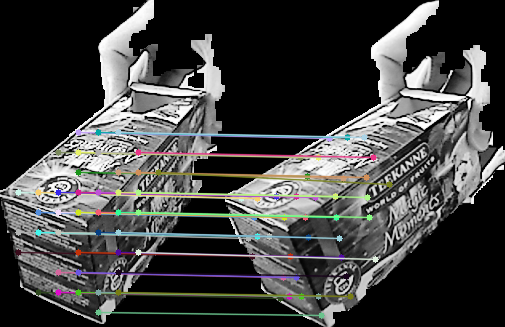
\includegraphics[width=300pt]{figures/vis_full.png}
\caption{Végső párosítás az optikai folyamok segítségével (16 841 vektor) \label{fig:vis_full}}
\end{figure}

%----------------------------------------------------------------------------
\section{Háromszögelés}
%----------------------------------------------------------------------------

Ahogy \aref{sec:triangulation}. alfejezetben bemutattam az elméleti hátteret, a következőkben ennek implementálását mutatom be.

\subsection{OpenCV-s függvényekkel}

OpenCV \texttt{cv::triangulatePoints} függvényben a \textit{Linear-LS} (lineáris legkisebb négyzetek) módszer van implementálva. Az interneten rákeresve több fórumban is találtam arra vonatkozó információkat, hogy sokan küzködnek ennek meghívásával. A dokumentáció \cite{camera-calib-3d} alapján sztereó-kalibráció során nyert projekciós mátrixokat várja a pontpárok mellett paraméterül. Az én esetemben, a kamerák nincsenek sztereó-kalibrálva, de a két projekciós mátrix megvan. Ennek ellenére a kimeneti 3D-s koordináták használhatatlanok voltak. Kis kutatás után az \texttt{cv::undistortPoints()} függvény meghívása jelentette a megoldást. Ez először normalizálta őket, vagyis:

\[\left(\begin{array}{c} u' \\ v' \\ 1 \end{array}\right) = {\underbrace{\left(\begin{array}{ccc}
f_x & 0 & o_x \\ 
0 & f_y & o_y \\
0 & 0 & 1
\end{array}\right)}_{\hbox{kamera-mátrix}}}^{-1} \left(\begin{array}{c} u \\ v \\ 1 \end{array}\right)\]

ahol $(u', v')$ az $(u, v)$ pont normalizáltja (kamera-mátrixtól független koordináták), majd a torzítási együtthatóakat felhasználva az $(u', v')$ pontoknak meghatározta a javított koordinátájukat. Ezután a \texttt{cv::triangulatePoints} függvénynek a projekciós mátrixok helyett csak az $\Big(\,\mathbf{R}\,|\,\mathbf{t}\,\Big)$ mátrixokat kellett átadnom. Fontos, hogy az előbbiekben kialakított pontpárosítás azon osztályához tartozó pontokat, melyek az eltolt képhez tartoznak, az eltoláshoz használt vektor ellentettjével vissza kell tolni, hogy valós koordinátákat kapjunk.

Miután megvannak a valóvilágbeli koordináták ezek pontosságát a képsíkokra történő visszavetítéssel vizsgáltam meg. A pontokat a \texttt{cv::projectPoints} függvénnyel vetítettem a bal oldali és jobb oldali kamera képére, majd a vetített és az eredeti pontok távolságainak átlagát -- átlagos visszavetítési hiba -- vizsgáltam. Ez az előzőekben mutatott bemenetre 8,68716 pixel lett, és \aref{fig:cv-triangulation}. ábrán látható az eredményeket bemutató két vizualizáció, melyeken a szín a pontok $z$ koordinátáját mutatja.

\begin{figure}[tbh]
\centering
\begin{subfigure}[b]{.49\linewidth}
	\centering
	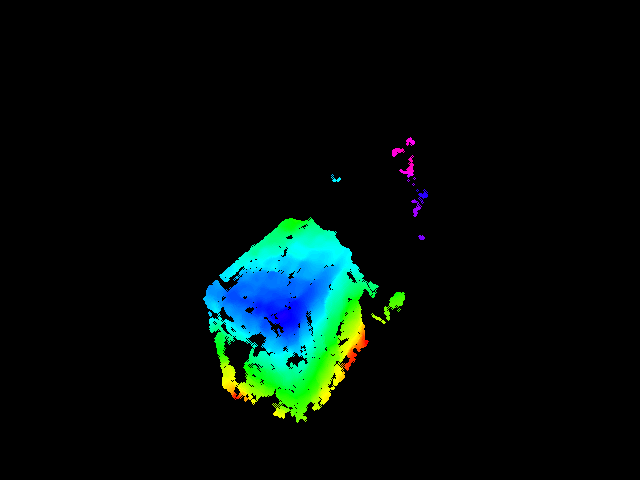
\includegraphics[width=205pt]{figures/visu_left.png}
	\caption{Bal oldali kamera nézőpontjából nézve \label{fig:cv-triangulation-a}}
  \end{subfigure}
\begin{subfigure}[b]{.49\linewidth}
	\centering
	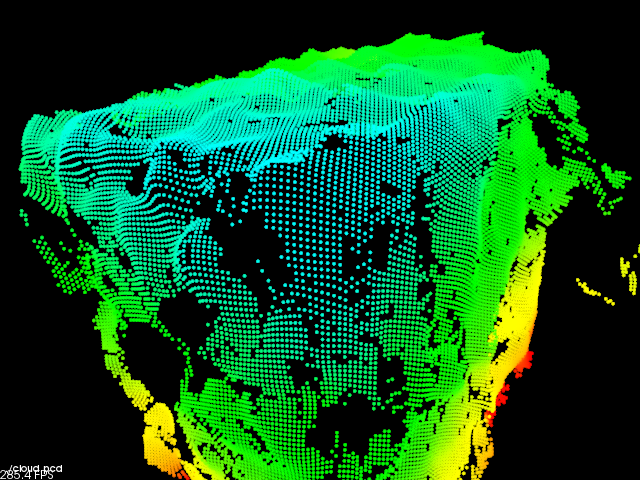
\includegraphics[width=205pt]{figures/visu_pcl.png}
	\caption{PCL vizualizációs szoftverrel ráközelítve}
  \end{subfigure}
\caption{Háromszögelés \textit{Linear-LS}-sel. Jól látható a közeli nézőpontból, hogy egy kissé hullámos lett a felület, de a pontatlanságra a hiba alapján számítottunk \label{fig:cv-triangulation}}
\end{figure}

Az OpenCV keretrendszerben megtalálhatjuk a \cite{hartley-triangulation}-ben leírt optimális, de polinomiális algoritmust is implementálva \texttt{cv::correctMatches()} néven, amely a fundamentális mátrix segítségével \aref{sec:triangulation}. szakaszban említett módon javítja a pontpárokat, azaz $\mathbf{u} \leftrightarrow \mathbf{u}'$ összerendelések helyett olyan $\mathbf{\hat{u}} \leftrightarrow \mathbf{\hat{u}}'$ párokat ad, melyekre $d(\mathbf{u}, \mathbf{\hat{u}})^2 + d(\mathbf{u}', \mathbf{\hat{u}}')^2$ minimális és teljesül, hogy $\mathbf{\hat{u}}'^T \mathbf{F} \mathbf{\hat{u}} = 0$. Ez az előbbi átlagos visszavetítési hibát 8,054 pixelre javította, de rohamos teljesítménycsökkenés mellett (0,06 másodperces futási idő helyett 0,64 másodperc lett, csak a háromszögelés), mely az eredményeket szabad szemmel megnézve nem meggyőző.


\subsection{Iteratív lineáris legkisebb négyzetek (\textit{Iterative-LS})}

\Aref{sec:triangulation}. szakaszban leírt iteratív módszert nem tudjuk alkalmazni a fenti \texttt{cv::triangulatePoints} függvénnyel, mert nem tudjuk az egyenleteket pontonként külön-külön súlyozni. Ennek megfelelően először a ,,szimpla'' \textit{Linear-LS} megközelítést kell implementálni, majd ezt már tudjuk majd iteratívan különböző súlyokkal meghívni.

Ehhez én Roy Shilkrot online elérhető alkalmazás-könyvtárából \cite{sfm-toy-library} merítettem a kiindulási alapot, és azt alakítottam az általam használt adatszerkezetekhez. Ehhez is előtte minden pontot normalizálni, valamint a torzítási együtthatóknak megfelelően javítani kellett. Ezzel a megközelítéssel 8,21 pixelnyi lett az átlagos visszavetítési hiba, de a sebesség harmadára csökkent (0,06 másodperc helyett 0,18 másodperc lett a futási idő), melyet szintén nem tekinthetünk kifizetődő kompromisszumnak.

A fentieket összegyűjtve a \texttt{Triangulator} osztályban (lásd \ref{fig:cd:triangulator}. ábra) implementáltam, melynek két metódusa a fent említett két módszert (OpenCV-s \texttt{triangulatePoints}, valamint az Iterative-LS) valósítja meg. Mindkettő az egymásnak megfelelő pontpárokat várja bemenetként, és harmadik paraméterében visszaadja az eredményt egy pontfelhőben, mely \texttt{CloudPoint}-ok vektoraként áll elő. Egy \texttt{CloudPoint} az aktuális koordinátákon kívül azt is tudja magáról, hogy mekkora a hozzátartozó visszavetítési hiba, így a megjelenítésnél eszerint tudunk is tudunk szűrni.

\begin{figure}[tbh]
\centering

\begin{tikzpicture} 

\begin{class}[text width=9.75 cm]{Triangulator}{0, 0}
\attribute{+ camera1 : Camera}
\attribute{+ camera2 : Camera}

\attribute{+ cameraPose1 : CameraPose}
\attribute{+ cameraPose2 : CameraPose}

\operation{+ triangulateIteratively(points1, points2, cloudpoints) : double}
\operation{+ triangulateCv(points1, points2, cloudpoints) : double}
\end{class}

\begin{class}[text width=3.5 cm]{CloudPoint}{7.75, 0}

\attribute{+ pt : Point3d}
\attribute{+ reprojErr : double}

\end{class}

\end{tikzpicture}

\caption{\texttt{Triangulator} osztály és \texttt{CloudPoint} struktúra \label{fig:cd:triangulator}}
\end{figure}

%----------------------------------------------------------------------------
\section{Változtatható nézőpont}
%----------------------------------------------------------------------------

Ahogy az előbbiekben (lásd \ref{fig:cv-triangulation-a}. ábra) már említettem, a \texttt{cv::projectPoints} függvény segítségével lehet meghatározni, hogy adott kamerából fényképezve a valóvilágbeli pontoknak hol vannak a vetületei. Háromféle megjelenítési technikát implementáltam; \begin{inparaenum}[\itshape 1\upshape)]
\item $z$ koordinátát jelölő színkód,
\item eredeti képpontok színeinek felhasználása és
\item kontúrok rajzolása.
\end{inparaenum}

Az első implementálását a HSV (hue, saturation, value) színtér segítségével valósítottam meg. $S$ és $V$ értékét fixen a maximumra állítottam, $H$ értékét pedig egyenletesen elosztottam a különböző $z$ koordináták mentén.

A másodikhoz a pontfelhő mellé még két információra volt szükség: a pontok koordinátáira a bal képen, valamint a bal képre, hogy a pixelek színeit ki tudjam nyerni. Ezek után az adott 3D-s pont vetített képpontjának a színét a balképen lévő forrás pixel színére állítottam.

A harmadik megoldást 3 lépésben valósítottam meg. Először fehér pontokként levetítettem a pontokat a képsíkra. Ezt követően dilatáció-erózió kombinációval morfológiai zárást hajtottam végre a bináris képen, minek köszönhetően a kisebb lyukak és szakadások megszűntek. Végül az eredményen kontúrokat kerestem a \texttt{cv::findContours()} függvény segítségével, és ezeket kirajzoltam. Egy határérték (amit 100 pixel$^2$-nek választottam) alatti területtel rendelkező kontúrokat elvetettem, mert ezek kisebb olyan foltokat jelentenek, melyeket nem tudunk egyértelműen egy nagyobb objektumhoz rendelni.

Ezen három vizualizációjának eredménye a bal oldali kamera nézpontjából látható \aref{fig:different-vis}. ábrán.

\begin{figure}[tbh]
\centering
\begin{subfigure}[b]{.33\linewidth}
	\centering
	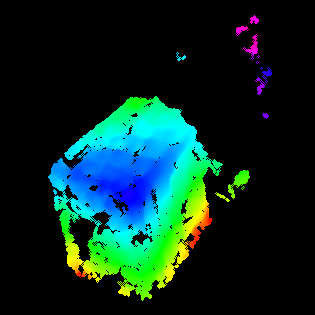
\includegraphics[width=135pt]{figures/visu_depth.png}
	\caption{Mélységinformáció}
  \end{subfigure}
\begin{subfigure}[b]{.32\linewidth}
	\centering
	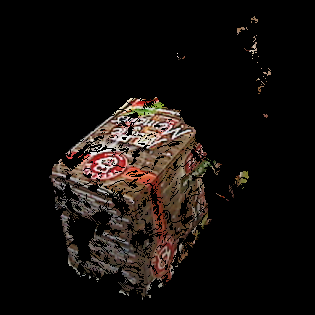
\includegraphics[width=135pt]{figures/visu_pixels.png}
	\caption{Eredeti pixelek}
  \end{subfigure}
\begin{subfigure}[b]{.32\linewidth}
	\centering
	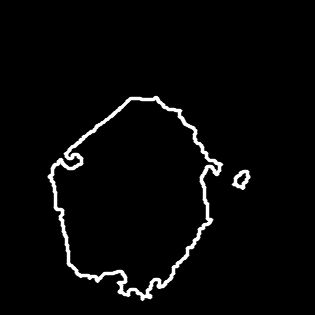
\includegraphics[width=135pt]{figures/visu_contours.png}
	\caption{Kontúrok}
  \end{subfigure}
\caption{Különböző vizualizációk, ráközelítve a hasznos területre \label{fig:different-vis}}
\end{figure}

Ahogy \aref{chapter3}. fejezetben említettem, a választott nézőpont, ahonnan érdemes lehet rekonstruálni az objektumot, a két kamera nézőpont között helyezkedhet el. Tehát a két kamera között szeretnénk interpolálni egy virtuális kamerát, és innen elvégezni a vetítést. Fontos, hogy nem elég csak a kamera helyzetét ($\mathbf{t_v}$), hanem a forgatási mátrixát ($\mathbf{R_v}$) is meg kell határozni. Jelölje $r \in [0; 1]$ a virtuális kamera pozícióját a pályáján, ahol $r = 0$, ha a bal oldali kamera, és $r = 1$, ha a jobb oldali kamera helyzetében van. Ekkor a virtuális kamera eltolási vektora $\mathbf{t_v} = (1-r)\mathbf{t_v} + r\mathbf{t_j}$, ahol $\mathbf{t_v}$ jelöli a bal oldali, $\mathbf{t_j}$ a jobb oldali kamera eltolási vektorát.
{\color{red} Kvaterniók...}

%----------------------------------------------------------------------------
\section{Párhuzamosítás, többszálúsítás}
%----------------------------------------------------------------------------


%----------------------------------------------------------------------------
\section{Eredmények, mérések, értékelés {\color{red} külön fejezet?}}
%----------------------------------------------------------------------------

